\section{The Kubernetes Cluster Autoscaler}\label{section:background_autoscaler}

There are three different types of autoscaling in Kubernetes:
\begin{itemize}
  \tightlist
  \item \textbf{Cluster Autoscaler (Autoscaler)}: adjusts the number of nodes in the
  cluster when Pods fail to schedule or when nodes are underutilized.
  \item \textbf{Horizontal Pod Autoscaler (HPA)}: adjusts the number of replicas
  of an application.
  \item \textbf{Vertical Pod Autoscaler (VPA)}: adjusts the resource requests and limits of the containers of a Pod.
\end{itemize}
\begin{figure}[ht]
  \centering
  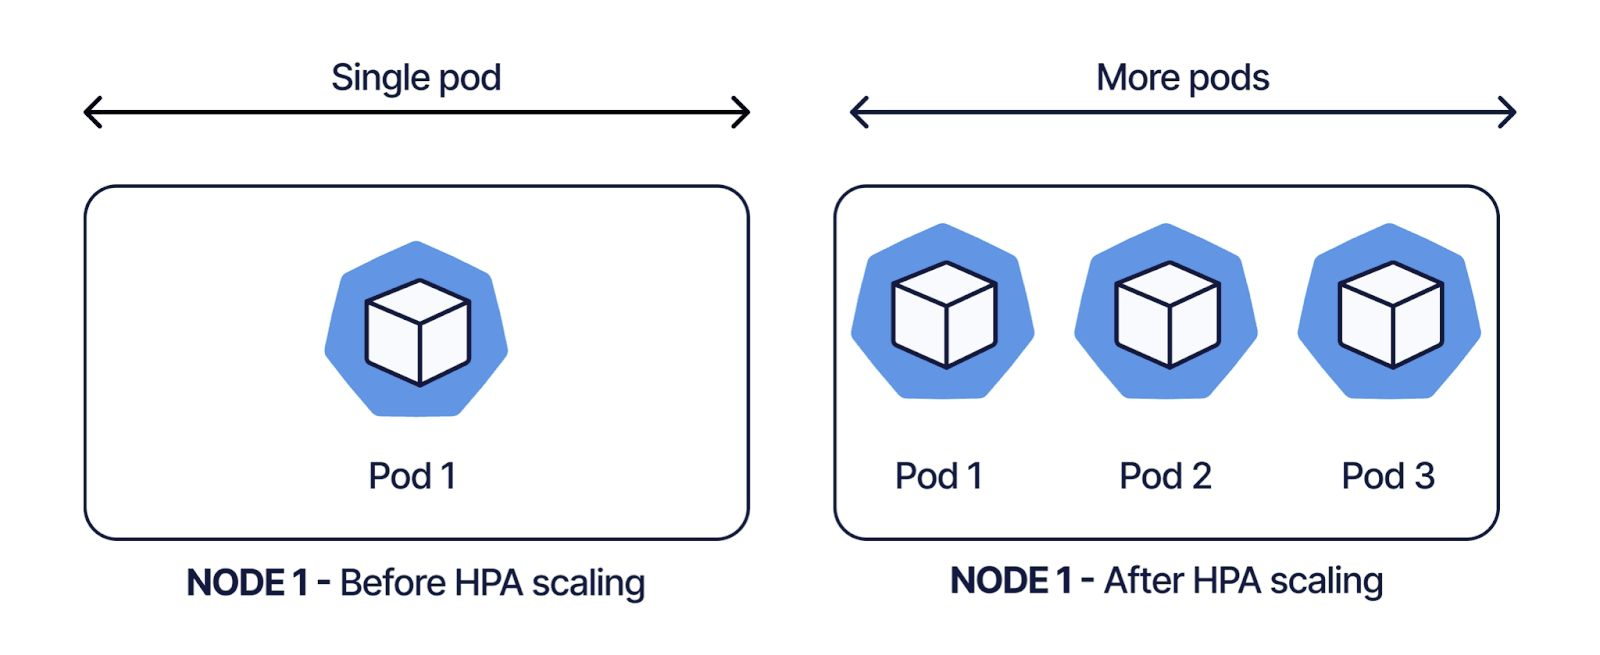
\includegraphics[width=0.9\textwidth]{resources/hpa-autoscaling-blue.png}
  \caption{Kubernetes Horizontal Pod Autoscaling}
\end{figure}

\begin{figure}[ht]
  \centering
  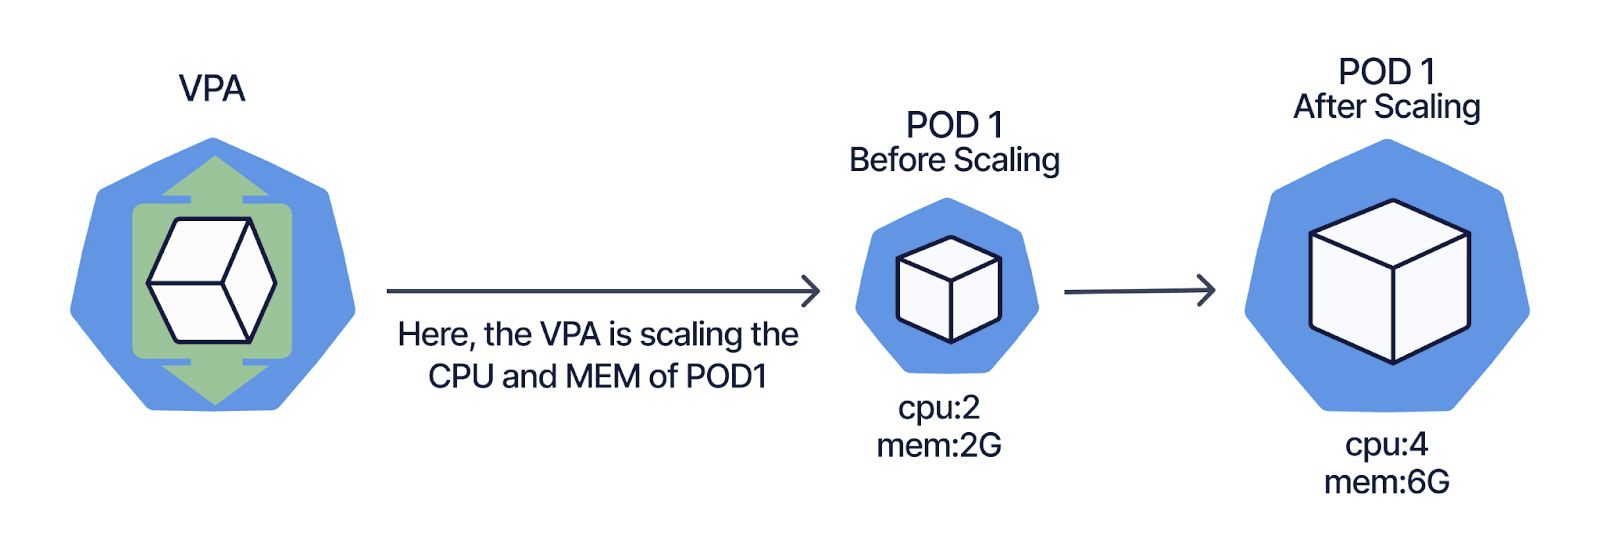
\includegraphics[width=0.9\textwidth]{resources/vpa-diagram-blue.png}
  \caption{Kubernetes Vertical Pod Autoscaling}
\end{figure}

\begin{figure}[ht]
  \centering
  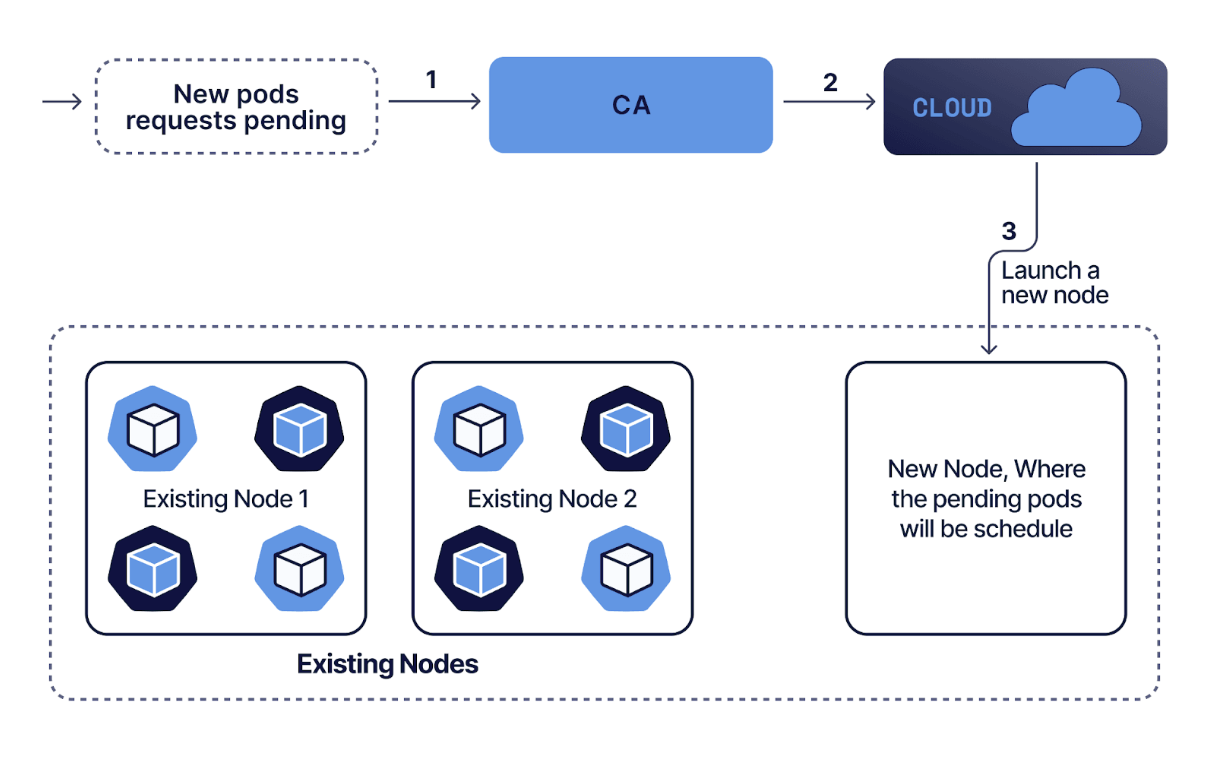
\includegraphics[width=0.9\textwidth]{resources/ca-process-blue.png}
  \caption{Kubernetes Cluster Autoscaling}
\end{figure}

%TODO: COLORBOX
\textbf{In the context of this thesis, we only discuss the Cluster Autoscaler. We will
refer to it as the ``Autoscaler'', and we will imply that we talk about the
Cluster Autoscaler.
}
\subsection{Cluster Autoscaling Fundamentals}

The Cluster Autoscaler is a component that automatically adjusts the Kubernetes
cluster size. It automatically adds or removes nodes based on the Pods' resource
requests compared to the nodes' available resources (see
section~\ref{section:pod-requests}); it does not measure the live CPU and memory
usage.

If the scheduler could not schedule any Pods, the Autoscaler will add new nodes
in the cluster to help the Pods get scheduled. This action is called
\textit{scale-up} of the cluster (or, equivalently, \textit{scale-out}). If any
nodes in the cluster are not needed, the Autoscaler will remove these nodes.
This action is called \textit{scale-down} of the cluster (or, equivalently,
\textit{scale-in}).

The following paragraphs explain the basic principles of scaling up and down a
cluster.

\subsection{Scale-Up Procedure}

\label{section:backgroud-scale-up}

The Autoscaler periodically checks for any unschedulable Pods on the cluster and
tries to find a new place for them to run.

The Autoscaler assumes that the underlying cluster runs on top of some
\textit{node groups}. Inside a node group, all machines have the same capacity
and assigned labels. Increasing the size of a node group will create a new node
that will be similar to those already in the cluster.

Based on the above assumption, the Autoscaler creates template nodes for each
node group and checks if any unschedulable Pod would fit on a new node. If there
are multiple node groups that, if increased, would help some Pods to run, the
administrator can specify different strategies for the Autoscaler to choose
which node group it shall increase. This procedure may require multiple
iterations before all the Pods are eventually scheduled.


\subsection{Scale-Down Procedure}
\label{section:backgroud-scale-down}

The Autoscaler periodically checks which nodes are unneeded, provided that no
scale-up is needed. A node is considered for removal if all the following
conditions hold:

\begin{itemize}
  \tightlist
  \item The sum of CPU and memory requests of all Pods running on this node is
  less than 50\% of the node's allocatable resources. This threshold is
  configurable.
  \item All Pods running on the node (except Pods created by Daemons) can be
  moved to any other node in the cluster. 
\end{itemize}

The Autoscaler removes a node if it remains unneeded for more than 10 minutes
(configurable duration). It terminates one \textit{non-empty} node at a time to
reduce the risk of creating new unschedulable Pods. On the other hand, it
terminates \textit{Empty} nodes (nodes that run only DaemonSet Pods) in bulk.
When a non-empty node is terminated, as mentioned above, all Pods should be
migrated elsewhere. It achieves this by marking the node unschedulable and then
evicting the Pods that run on it. As soon as each Pod is successfully evicted,
the scheduler shall schedule it on a different node.
